\begin{figure}
\centering
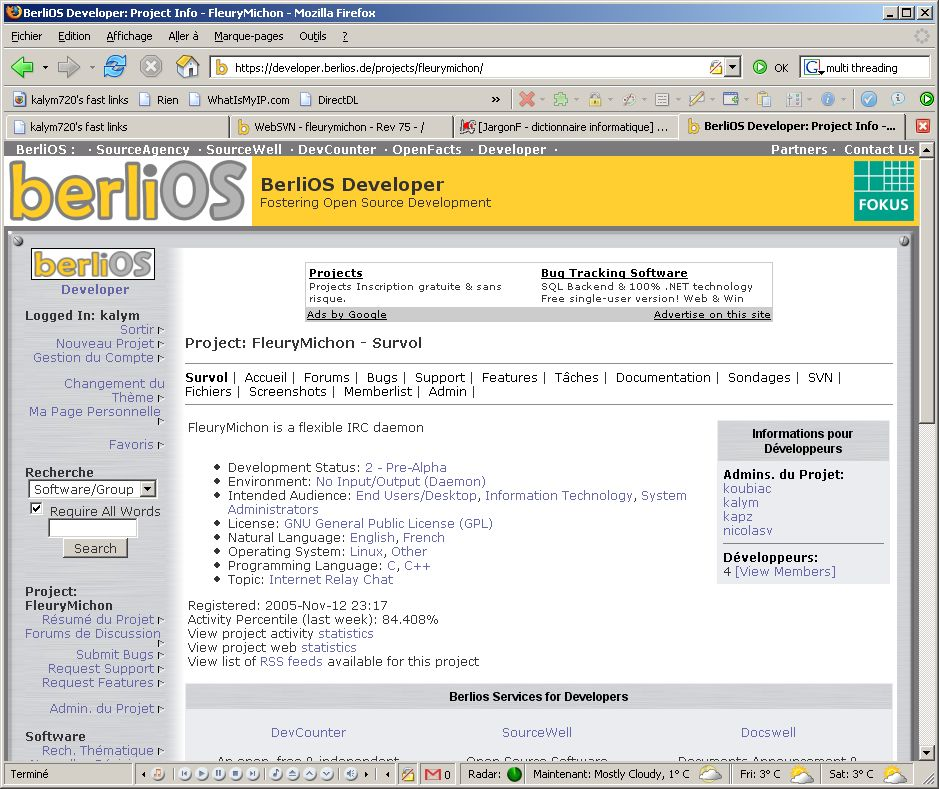
\includegraphics[width=.8\linewidth]{berlios.jpg}
\caption{Page d'accueil du projet}
\end{figure}

\begin{figure}
\centering
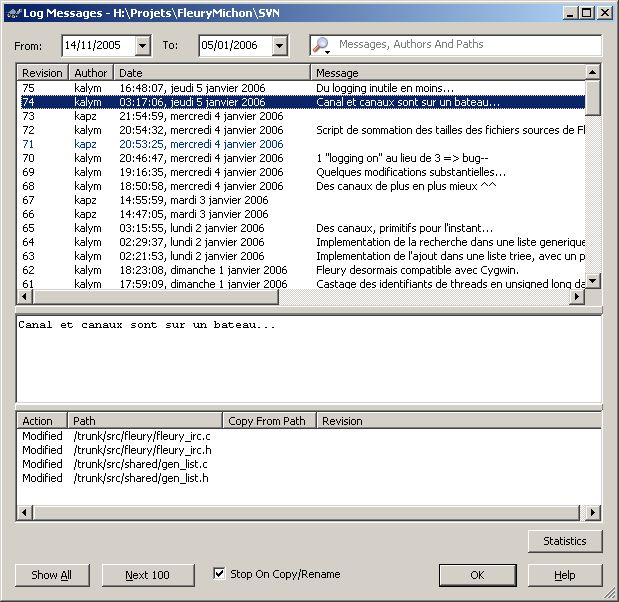
\includegraphics[width=.8\linewidth]{svn_log.jpg}
\caption{TortoiseSVN sous Windows}
\end{figure}

\begin{figure}
\centering
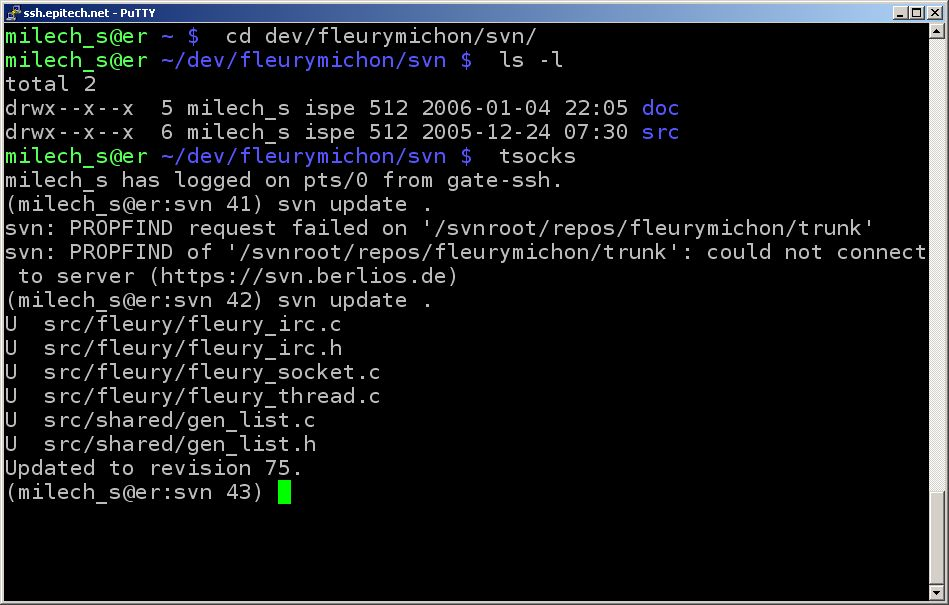
\includegraphics[width=.8\linewidth]{svn_ssh_update.jpg}
\caption{svn sous Linux, avec le proxy qui marche une fois sur deux}
\end{figure}

\begin{figure}
\centering
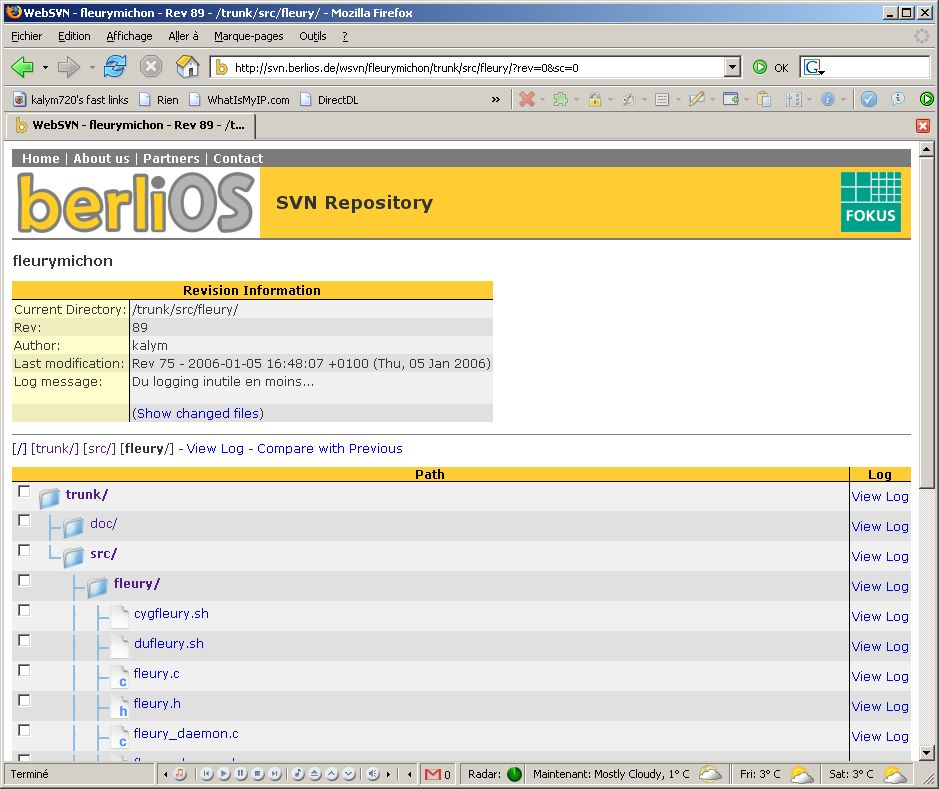
\includegraphics[width=.8\linewidth]{websvn.jpg}
\caption{Le WebSVN}
\end{figure}

\section{Site Web}

Notre projet est h�berg� chez BerliOS, il s'agit d'un fournisseur de services pour d�veloppeurs qui nous apporte d'innombrables outils pour travailler sur notre projet. Nous disposons d'une interface assez compl�te permettant d'organiser l'�volution du projet, nous pouvons recevoir des demandes d'ajout de fonctionnalit�s, des demandes de support, �mettre des sondages, rapporter les bugs, discuter, publier les releases du projet, des screenshots, de la documentation \ldots 
La page d'accueil est accessible � l'adresse : (\textit{Voir Fig 4.1})\\
\verb+http://developer.berlios.de/projects/fleurymichon/+ \\

\section{Repository}

Par ailleurs, BerliOS nous offre �galement un repository Subversion. Il s'agit d'un gestionnaire de code source, qui nous permet de synchroniser notre travail � la fois rapidement et efficacement. \\
TortoiseSVN, un client graphique qui s'int�gre � l'explorateur Windows est disponible gratuitement (\textit{Voir Fig 4.2}).
Les utilitaires svn et svnadmin sont disponibles avec la majorit� des distributions Linux (\textit{Voir Fig 4.3}). Le WebSVN accessible � l'URL : \\
\verb+http://svn.berlios.de/wsvn/fleurymichon/+ \\
permet de consulter les fichiers sources du projet � partir de n'importe quel navigateur (\textit{Voir Fig 4.4}).
